\documentclass[10pt,a4paper]{article}
\usepackage[right=0.5cm, left=0.5cm,top=0.5cm,bottom=0.5cm]{geometry}
\usepackage{enumitem}
\usepackage{forest}
\usepackage{amsfonts}
\usepackage{tikz}
\usetikzlibrary{positioning}
\usepackage{graphicx}
\usepackage{array, tasks}
\usepackage{blindtext}
\usepackage{fontspec}
\usepackage{amsmath,amsfonts,amssymb,mathrsfs,amsthm}
\usepackage{fancyhdr}
\usepackage{xcolor}
\usepackage{booktabs}
\usepackage[font={bf}]{caption}
% \captionsetup[table]{box=colorbox,boxcolor=orange!20}
\usepackage{float}
\usepackage{esvect}
\usepackage{tabularx}
\usepackage{pifont}
\usepackage{colortbl}
 \usepackage{fancybox}
 \mathversion{bold}
 \usepackage{pgfplots}
 % \usepackage[utf8]{inputenc}
\usepackage{tikz}
 \usepackage[tikz]{bclogo}%
 \usepackage{mathpazo}
\usepackage{ulem}
\usepackage{yagusylo}
\usepackage{textcomp}\usepackage{blindtext}
\usepackage{multicol}
\usepackage{varwidth}
\usetikzlibrary{calc,intersections}
\usepackage{pgfplots}
%\usepackage{fourier}
\pgfplotsset{compat=1.11}
\usepackage{tkz-tab}
\usepackage{xcolor}
\usepackage{color}
\usetikzlibrary{calc}
\mathchardef\times="2202
\usepackage[most]{tcolorbox}
\definecolor{lightgray}{gray}{0.9}
\definecolor{ocre}{RGB}{0,244,244} 
\definecolor{head}{RGB}{255,211,204}
\definecolor{browndark}{RGB}{105,79,56}
%\RequirePackage[framemethod=default]{mdframed}
\usepackage{tikz}
\usetikzlibrary{calc,patterns,decorations.pathmorphing,arrows.meta,decorations.markings}
\usetikzlibrary{arrows.meta}
\makeatletter
\tcbuselibrary{skins,breakable,xparse}
\tcbset{%
  save height/.code={%
    \tcbset{breakable}%
    \providecommand{#1}{2cm}%
    \def\tcb@split@start{%
      \tcb@breakat@init%
      \tcb@comp@h@page%
      \def\tcb@ch{%
        \tcbset{height=\tcb@h@page}%
        \tcbdimto#1{#1+\tcb@h@page-\tcb@natheight}%
        \immediate\write\@auxout{\string\gdef\string#1{#1}}%
        \tcb@ch%
      }%
      \tcb@drawcolorbox@standalone%
    }%
  }%
}
\newcommand{\Lim}{\displaystyle\lim}
\makeatother
\newcommand{\oij}{$\left( \text{O};\vv{i},\vv{j} , \vv{k}\right)$}
\colorlet{darkred}{red!30!black}
\newcommand{\red}[1]{\textcolor{darkred}{ #1}}
\newcommand{\rr}{\mathbb{R}}
\renewcommand{\baselinestretch}{1.2}
 \setlength{\arrayrulewidth}{1.25pt}
\usepackage{titlesec}
\usepackage{titletoc}
\usepackage{minitoc}
\usepackage{ulem}
%--------------------------------------------------------------

\usetikzlibrary{decorations.pathmorphing}
\tcbuselibrary{skins}

%%%%%%%%%%%
%-------------------------------------------------------------------------
\tcbset{
        enhanced,
        colback=white,
        boxrule=0.1pt,
        colframe=brown!10,
        fonttitle=\bfseries
       }
\definecolor{problemblue}{RGB}{100,134,158}
\definecolor{idiomsgreen}{RGB}{0,162,0}
\definecolor{exercisebgblue}{RGB}{192,232,252}
\definecolor{darkbrown}{rgb}{0.4, 0.26, 0.13}

\newcommand*{\arraycolor}[1]{\protect\leavevmode\color{#1}}
\newcolumntype{A}{>{\columncolor{blue!50!white}}c}
\newcolumntype{B}{>{\columncolor{LightGoldenrod}}c}
\newcolumntype{C}{>{\columncolor{FireBrick!50}}c}
\newcolumntype{D}{>{\columncolor{Gray!42}}c}

\newcounter{mysection}
\newcounter{mysubsection}
\newcommand{\mysection}[1]{%
    \stepcounter{mysection} % Increment the counter
    \textcolor{red}{\LARGE\themysection. #1 :}
}
\newcommand{\mysubsection}[2]{
    \stepcounter{mysubsection}
    \textcolor{red}{\large \themysection.#1. #2 :}
}
% \textcolor{red}{\LARGE\bfseries 1. Les équation du deuxiéme degrée :}

%------------------------------------------------------
\newtcolorbox[auto counter]{Definition}{enhanced,
before skip=2mm,after skip=2mm,
colback=yellow!20!white,colframe=lime,boxrule=0.2mm,
attach boxed title to top left =
    {xshift=0.6cm,yshift*=1mm-\tcboxedtitleheight},
    varwidth boxed title*=-3cm,
    boxed title style={frame code={
                        \path[fill=lime]
                            ([yshift=-1mm,xshift=-1mm]frame.north west)  
                            arc[start angle=0,end angle=180,radius=1mm]
                            ([yshift=-1mm,xshift=1mm]frame.north east)
                            arc[start angle=180,end angle=0,radius=1mm];
                        \path[left color=lime,right color = lime,
                            middle color = lime]
                            ([xshift=-2mm]frame.north west) -- ([xshift=2mm]frame.north east)
                            [rounded corners=1mm]-- ([xshift=1mm,yshift=-1mm]frame.north east) 
                            -- (frame.south east) -- (frame.south west)
                            -- ([xshift=-1mm,yshift=-1mm]frame.north west)
                            [sharp corners]-- cycle;
                            },interior engine=empty,
                    },
fonttitle=\bfseries\sffamily,
title={Definition ~\thetcbcounter}}
%------------------------------------------------------
\newtcolorbox[auto counter]{Proposition}{enhanced,
before skip=2mm,after skip=2mm,
colback=yellow!20!white,colframe=blue,boxrule=0.2mm,
attach boxed title to top left =
    {xshift=0.6cm,yshift*=1mm-\tcboxedtitleheight},
    varwidth boxed title*=-3cm,
    boxed title style={frame code={
                        \path[fill=blue]
                            ([yshift=-1mm,xshift=-1mm]frame.north west)  
                            arc[start angle=0,end angle=180,radius=1mm]
                            ([yshift=-1mm,xshift=1mm]frame.north east)
                            arc[start angle=180,end angle=0,radius=1mm];
                        \path[left color=blue,right color = blue,
                            middle color = blue]
                            ([xshift=-2mm]frame.north west) -- ([xshift=2mm]frame.north east)
                            [rounded corners=1mm]-- ([xshift=1mm,yshift=-1mm]frame.north east) 
                            -- (frame.south east) -- (frame.south west)
                            -- ([xshift=-1mm,yshift=-1mm]frame.north west)
                            [sharp corners]-- cycle;
                            },interior engine=empty,
                    },
fonttitle=\bfseries\sffamily,
title={Proposition ~\thetcbcounter}}
%------------------------------------------------------
\newtcolorbox[auto counter]{Thm}[1]{enhanced,
before skip=2mm,after skip=2mm,
colback=yellow!20!white,colframe=red,boxrule=0.2mm,
attach boxed title to top left =
    {xshift=0.6cm,yshift*=1mm-\tcboxedtitleheight},
    varwidth boxed title*=-3cm,
    boxed title style={frame code={
                        \path[fill=red]
                            ([yshift=-1mm,xshift=-1mm]frame.north west)  
                            arc[start angle=0,end angle=180,radius=1mm]
                            ([yshift=-1mm,xshift=1mm]frame.north east)
                            arc[start angle=180,end angle=0,radius=1mm];
                        \path[left color=red,right color = red,
                            middle color = red]
                            ([xshift=-2mm]frame.north west) -- ([xshift=2mm]frame.north east)
                            [rounded corners=1mm]-- ([xshift=1mm,yshift=-1mm]frame.north east) 
                            -- (frame.south east) -- (frame.south west)
                            -- ([xshift=-1mm,yshift=-1mm]frame.north west)
                            [sharp corners]-- cycle;
                            },interior engine=empty,
                    },
fonttitle=\bfseries\sffamily,
title={#1 ~\thetcbcounter}}
%------------------------------------------------------
\newtcolorbox[auto counter]{exemple}{
  % breakable,
  enhanced,
  colback=white,
  boxrule=0pt,
  arc=0pt,
  outer arc=0pt,
  title=Exemple ~\thetcbcounter,
  fonttitle=\bfseries\sffamily\large\strut,
  coltitle=problemblue,
  colbacktitle=problemblue,
  title style={
left color=exercisebgblue,
    right color=white,
    middle color=exercisebgblue  
  },
  overlay={
    \draw[line width=1pt,problemblue] (frame.south west) -- (frame.south east);
    \draw[line width=1pt,problemblue] (frame.north west) -- (frame.north east);
    \draw[line width=1pt,problemblue] (frame.south west) -- (frame.north west);
    \draw[line width=1pt,problemblue] (frame.south east) -- (frame.north east);
  }
}
%----------------------------------------------------
\newtcolorbox[auto counter]{application}{
  % breakable,
  enhanced,
  colback=white,
  boxrule=0pt,
  arc=0pt,
  outer arc=0pt,
  title=Application ~\thetcbcounter,
  fonttitle=\bfseries\sffamily\large\strut,
  coltitle=problemblue,
  colbacktitle=problemblue,
  title style={
left color=exercisebgblue,
    right color=white,
    middle color=exercisebgblue  
  },
  overlay={
    \draw[line width=1pt,problemblue] (frame.south west) -- (frame.south east);
    \draw[line width=1pt,problemblue] (frame.north west) -- (frame.north east);
    \draw[line width=1pt,problemblue] (frame.south west) -- (frame.north west);
    \draw[line width=1pt,problemblue] (frame.south east) -- (frame.north east);
  }
}
%----------------------------------------------------
\newtcolorbox[auto counter]{Activite}{
  % breakable,
  enhanced,
  colback=white,
  boxrule=0pt,
  arc=0pt,
  outer arc=0pt,
  title=Activité ~\thetcbcounter,
  fonttitle=\bfseries\sffamily\large\strut,
  coltitle=problemblue,
  colbacktitle=problemblue,
  title style={
left color=yellow!50!white,
    right color=white,
    middle color=yellow!20!white  
  },
  overlay={
    \draw[line width=1pt,problemblue] (frame.south west) -- (frame.south east);
    \draw[line width=1pt,problemblue] (frame.north west) -- (frame.north east);
    \draw[line width=1pt,problemblue] (frame.south west) -- (frame.north west);
    \draw[line width=1pt,problemblue] (frame.south east) -- (frame.north east);
  }
}
%---------------------------------------------
\newtcolorbox{mybox}[2]{enhanced,breakable,
    before skip=2mm,after skip=2mm,
    colback=white,colframe=#2!30!blue,boxrule=0.3mm,rightrule=0.3mm,
    attach boxed title to top center={xshift=0cm,yshift*=1mm-\tcboxedtitleheight},
    varwidth boxed title*=-3cm,
    boxed title style={frame code={
    \path[fill=#2!30!black]
    ([yshift=-1mm,xshift=-1mm]frame.north west)
    arc[start angle=0,end angle=180,radius=1mm]
    ([yshift=-1mm,xshift=1mm]frame.north east)
    arc[start angle=180,end angle=0,radius=1mm];
    \path[draw=black,line width=1pt,left color=#2!1!white,right color=#2!1!blue!65,
    middle color=#2!1!green]
    ([xshift=-2mm]frame.north west) -- ([xshift=2mm]frame.north east)
    [rounded corners=1mm]-- ([xshift=1mm,yshift=-1mm]frame.north east)
    -- (frame.south east) -- (frame.south west)
    -- ([xshift=-1mm,yshift=-1mm]frame.north west)
    [sharp corners]-- cycle;
    },interior engine=empty,
    },
title=#1,coltitle=black,fonttitle=\sffamily}
%---------------------------------------------
\newtcolorbox{boxone}{%
    enhanced,
    colback=brown!10,
    boxrule=0pt,
    sharp corners,
    drop lifted shadow,
    frame hidden,
    fontupper=\bfseries,
    notitle,
    overlay={%
        \draw[Circle-Circle, brown!70!black, line width=2pt](frame.north west)--(frame.south west); 
        \draw[Circle-Circle, brown!70!black, line width=2pt](frame.north east)--(frame.south east);}
    }

    \tikzset{ midd/.style={
decoration={
markings,
mark=at position 0.5 with {%
\makebox[4pt][r]{\arrow{triangle 45}},
},
},
postaction={decorate},{Circle[]}-{Circle[]}
},}%
\tikzset{ midd/.style={
decoration={
markings,
% mark=at position 0.5 with {%
% \makebox[4pt][r]{\arrow{triangle 45}},
% },
},
% postaction={decorate},{Circle[]}-{Circle[]}
},}%
    
\begin{document}

\begin{tcolorbox}[title=\textcolor{blue}{\shadowbox{ Prof : Othmane Laksoumi}}
\hfill
\textcolor{blue}{\shadowbox{ Dérivation et étude de fonction numériques }}]

\end{tcolorbox}

\begin{mybox}{Lycée Qualifiant Zitoun}{gray}
    \begin{minipage}{8cm}
    \textcolor{darkbrown}{Année scolaire : } 2024-2025 \\
    \textcolor{darkbrown}{Niveau : } 2 Bac Sciences Physiques \\
    \textcolor{darkbrown}{Durée totale : } $10h$
    \end{minipage}
\end{mybox}

\begin{boxone}
{\Large\ding{45}}
\textcolor{red}{\large Contenus du programme :}
\begin{itemize}
    \item Continuité et dérivabilité.
    \item Dérivabilité de la composée de deux fonctions dérivables.
    \item Dérivée de la fonction réciproque.
    \item Dérivée de la fonction $x\mapsto \sqrt[n]{x}\ (n\geq 1)$.
    \item Exemples d'études de fonctions.
\end{itemize}

{\Large\ding{45}}
\textcolor{red}{\large Les capacités attendues :}
\begin{itemize}
    \item Calculer les dérivées des fonctions usuelles.
    \item Déterminer la monotonie d'une fonction à partir de son tableau de variation ou de sa représentation graphique.
    \item Résoudre graphiquement des équations de la forme $f(x) = g(x)$ et des inéquations de la forme $f(x) \leq g(x)$.
    \item Déterminer la monotonie de la fonction réciproque d'une fonction continue et strictement monotone et représenter graphiquement la fonction réciproque.
    \item Déterminer le nombre dérivé de la fonction réciproque d'une fonction en un point.
    \item Résoudre des problémes concernant les valeurs miminales et valeurs maximales.
    \item Étudier et représenter des fonctions ratinnelles et des fonctions trigonométriques.
\end{itemize}

{\Large\ding{45}}
\textcolor{red}{\large Recommandations pédagogiques :} 
  \begin{itemize}
    \item On rappellera la notion de dérivation et ses applications à partir d’activités variées faisant apparaître son importance dans l’étude locale et globale des fonctions au programme surtout l’approximation locale d’une fonction, l’étude du sens de variation d’une fonction sur un intervalle, la détermination des extrema et l’étude du signe d’une fonction ou d’une égalité algébrique sur un intervalle ou la concavité de la courbe d’une fonction numérique..., ce sera également une occasion pour rappeler la propriété caractéristique d’une fonction constante ou strictement monotone sur un intervalle.
    \item Les fonctions réciproques des fonctions trigonométriques usuelles sont hors programme.
    \item À partir de l’étude d’exemples de fonctions polynômes, de fonctions rationnelles, de fonctions trigonométriques et de fonctions irrationnelles on maintiendra les acquis des élèves relatifs à la dérivation, aux limites, à l’approximation par une fonction linéaire, aux éléments de symétrie de la courbe d’une fonction, à l’étude des branches infinies et à la résolution graphique de quelques équations et inéquations .......
    \item On se limitera à l'étude de quelques exemples de fonctions irrationnelles dont le signe de la dérivée ne pose pas de difficulté; à cette eccasion on abordera les équations irrationnelles à partir d'exemples.
    \item Utiliser l'écriture différentielle $dy = f^{\prime}(x)dx$.
    \item L'étude des fonctions de la forme $x\mapsto \sqrt[n]{u(x)}$ où $(n\geq 3)$ et $u$ une fonction positive, est hors programme, toutefois on se limitera à la détermination de leurs dérivées.
  \end{itemize}
\end{boxone}


\begin{tabular}{|>{\raggedright\arraybackslash}p{17cm}|>{\centering\arraybackslash}p{0.8cm}|}
\hline
\rowcolor{head}

\centering Contenu du cour &
 Durée \\
\hline
 
\vspace{1mm}
\mysection{Dérivabilité d'une fonction numérique (Rappels)}

\mysubsection{1}{Dérivabilité  d'une fonction en un point}
\begin{Definition}
    Soit $f$ une fonction numérique définie sur un intervalle ouvert $I$ et $x_0\in I$.
    On dit que $f$ est dérivable en $x_0$ s'il existe un réel $l$ tel que : $\Lim_{x\to x_0}\displaystyle\frac{f(x) - f(x_0)}{x - x_0} = l.$

    Le nombre $l$ est appelé \textcolor{red}{le nombre dérivé} de la fonction $f$ en $x_0$. Il est noté $f^{\prime}(x_0)$.
\end{Definition}

\textcolor{red}{Remarque :}

$$f^{\prime}(x_0) = \Lim_{x\to x_0}\displaystyle\frac{f(x) - f(x_0)}{x - x_0} = \Lim_{h\to 0}\displaystyle\frac{f(x_0 + h) - f(x_0)}{h}$$
\begin{Definition}
    Soit $f$ une fonction dérivable en $x_0$.

    La droite $(T)$ d'équation $y = f^{\prime}(x_0)(x-x_0) + f(x_0)$ est appelée la tangente à la courbe $\mathcal{C}_f$ de la fonction $f$ au point d'abscisse $x_0$.

    La fonction $x\mapsto f^{\prime}(x_0)(x-x_0) + f(x_0)$ s'appelle \textcolor{red}{l'approximation affine} de $f$ au voisinage de $x_0$.

    On écrit alors : $f(x)\approx f^{\prime}(x_0)(x-x_0) + f(x_0)$ au voisinage de $x_0$.
\end{Definition}
\begin{center}
	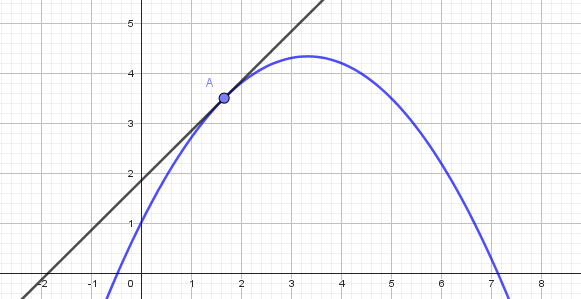
\includegraphics[width = 0.5\textwidth]{tangente.PNG}
\end{center}
\mysubsection{2}{Dérivation à droite - Dérivation à gauche}
\begin{Definition}
    \begin{itemize}
        \item Soit $f$ une fonction définie sur un intervalle du type $[x_0, x_0 + r[$ où $r\in\mathbb{R}^*_+$.

        On dit que $f$ est dérivable à droite de $x_0$ s'il existe  un réel $l_1$ tel que : $ \Lim_{x\to x_0^+}\displaystyle\frac{f(x) - f(x_0)}{x - x_0} = l_1$.
        On note $f^{\prime}_d(x_0) =  \Lim_{x\to x_0^+}\displaystyle\frac{f(x) - f(x_0)}{x - x_0}$
        \item Soit $f$ une fonction définie sur un intervalle du type $]x_0 - r, x_0]$ où $r\in\mathbb{R}^*_+$.

         On dit que $f$ est dérivable à gauche de $x_0$ s'il existe  un réel $l_2$ tel que : $ \Lim_{x\to x_0^-}\displaystyle\frac{f(x) - f(x_0)}{x - x_0} = l_2$.
        On note $f^{\prime}_g(x_0) =  \Lim_{x\to x_0^-}\displaystyle\frac{f(x) - f(x_0)}{x - x_0}$
    \end{itemize}
\end{Definition}

\begin{Proposition}
    Soit $f$ une fonction définie sur un intervalle ouvert $I$ et $x_0\in I$.

    La fonction $f$ est dérivable en $x_0$ si, et seulement si, elle est dérivable à droite et à gauche en $x_0$, avec $f^{\prime}_d(x_0) = f^{\prime}_g(x_0)$, et dans ce cas : $f^{\prime}(x_0) = f^{\prime}_d(x_0) = f^{\prime}_g(x_0)$.
\end{Proposition}


&\\
\hline
\end{tabular}

\begin{tabular}{|>{\raggedright\arraybackslash}p{17cm}|>{\centering\arraybackslash}p{0.8cm}|}
\hline

\vspace{1mm}
\begin{exemple}
    On considére la fonction $f$ définie sur $\mathbb{R}$ par :
    $$\begin{cases}
        f(x) = x - 3\sqrt[3]{x - 1} \quad;\quad x\geq 1 \\
        f(x) = \displaystyle\frac{1}{\sqrt{x}} \quad;\quad x < 1
    \end{cases}$$
    Étudions la dérivabilité de la fonction $f$ au point $x_0 = 1$.
\end{exemple}

\mysubsection{3}{Les interprétations géométriques} 

\begin{tabular}{|>{\centering}m{0.3\textwidth}|m{0.5\textwidth}|}
\hline
    Limite &  Interprétation géométrique \\
    \hline
     $\Lim_{x\to x_0}\displaystyle\frac{f(x) - f(x_0)}{x - x_0} = l$ & $(\mathcal{C}_f)$  admet une tangente d'équation : 
     
     $y = f^{\prime}(x_0)(x-x_0) + f(x_0)$ au point d'abscisse $x_0$.\\
\hline     
    $\Lim_{x\to x_0^+}\displaystyle\frac{f(x) - f(x_0)}{x - x_0} = l$ & $(\mathcal{C}_f)$  admet une demi-tangente d'équation : 
     $\begin{cases}
         y = f^{\prime}_d(x_0)(x-x_0) + f(x_0) \\
         x\geq x_0
     \end{cases}$
      au point d'abscisse $x_0$.\\
\hline
     $\Lim_{x\to x_0^-}\displaystyle\frac{f(x) - f(x_0)}{x - x_0} = l$ & $(\mathcal{C}_f)$  admet une demi-tangente d'équation : 
     $\begin{cases}
         y = f^{\prime}_d(x_0)(x-x_0) + f(x_0) \\
         x\leq x_0
     \end{cases}$
      au point d'abscisse $x_0$.\\
\hline
    $\Lim_{x\to x_0}\displaystyle\frac{f(x) - f(x_0)}{x - x_0} = 0$ & $(\mathcal{C}_f)$ admet une tangente horizontale au point d'abscisse $x_0$.\\
\hline
 $\Lim_{x\to x_0^+}\displaystyle\frac{f(x) - f(x_0)}{x - x_0} = +\infty$ & $(\mathcal{C}_f)$  admet une demi-tangente vertical dirigée vers le haut au point d'abscisse $a$.\\
\hline
$\Lim_{x\to x_0^+}\displaystyle\frac{f(x) - f(x_0)}{x - x_0} = -\infty$ & $(\mathcal{C}_f)$  admet une demi-tangente vertical dirigée vers le bas au point d'abscisse $a$.\\
\hline
$\Lim_{x\to x_0^-}\displaystyle\frac{f(x) - f(x_0)}{x - x_0} = +\infty$ & $(\mathcal{C}_f)$  admet une demi-tangente vertical dirigée vers le haut au point d'abscisse $a$.\\
\hline
$\Lim_{x\to x_0^-}\displaystyle\frac{f(x) - f(x_0)}{x - x_0} = -\infty$ & $(\mathcal{C}_f)$  admet une demi-tangente vertical dirigée vers le bas au point d'abscisse $a$.\\
\hline
\end{tabular}
\vspace{1mm}

\mysubsection{4}{Dérivabilité d'une fonction sur un intervalle}
\newline\newline
\begin{tabular}{|>{\centering}m{0.3\textwidth}|>{\centering}m{0.2\textwidth}|>{}m{0.25\textwidth}|}
\hline
    La fonction $f$ & La fonction $f^{\prime}$ & Domaine de dérivabilité\\
\hline
     $x\mapsto c \ (c\in\mathbb{R})$ & $x\mapsto 0$ & $\mathbb{R}$ \\
\hline
     $x\mapsto ax \ (a\in\mathbb{R})$ & $x\mapsto a$ & $\mathbb{R}$ \\
\hline
     $x\mapsto x^n$ & $x\mapsto nx^{n-1}$ & $\mathbb{R}$ \\
\hline
     $x\mapsto \displaystyle\frac{1}{x}$ & $x\mapsto -\displaystyle\frac{1}{x^2}$ & $\mathbb{R}^*$ \\
\hline
     $x\mapsto \sqrt{x}$ & $x\mapsto \displaystyle\frac{1}{2\sqrt{x}}$ & $\mathbb{R}^*_+$ \\
\hline
     $x\mapsto \sin{x}$ & $x\mapsto\cos{x}$ & $\mathbb{R}$ \\
\hline
     $x\mapsto \cos{x}$ & $x\mapsto-\sin{x}$ & $\mathbb{R}$ \\
\hline
     $x\mapsto \tan{x}$ & $x\mapsto 1 + \tan{x} = \displaystyle\frac{1}{\cos^2{x}}$ & $\left]-\displaystyle\frac{\pi}{2} + k\pi;\displaystyle\frac{\pi}{2} + k\pi\right[ \ (k\in\mathbb{Z})$ \\
\hline
     $x\mapsto \sin(ax + b) \ (a,b\in\mathbb{R})$ & $x\mapsto a\cos(ax + b)$ & $\mathbb{R}$ \\
\hline
     $x\mapsto \cos(ax + b) \ (a,b\in\mathbb{R})$ & $x\mapsto -a\sin(ax + b)$ & $\mathbb{R}$ \\
\hline
\end{tabular}

&\\
\hline
\end{tabular}


\begin{tabular}{|>{\raggedright\arraybackslash}p{17cm}|>{\centering\arraybackslash}p{0.8cm}|}
\hline

\vspace{1mm}
\mysubsection{5}{Opérations sur les fonctions dérivables}
\begin{Proposition}
    Soit $f$ et $g$ deux fonctions dérivables sur un intervalle $I$ et $\alpha\in\mathbb{R}$. Alors :
    $$(f + g)^{\prime} = f^{\prime} + g^{\prime} \quad;\quad (\alpha.f)^{\prime} =\alpha.f^{\prime} \quad;\quad (f.g)^{\prime} = f^{\prime}.g + f.g^{\prime} \quad;\quad (f^n)^{\prime} = n.f^{\prime}.f^{n-1}$$
    Si la fonction $g$ ne s'annule pas sur $I$, alors : $\left(\displaystyle\frac{1}{g}\right)^{\prime} = -\displaystyle\frac{g}{g^2}$ et $\left(\displaystyle\frac{f}{g}\right)^{\prime} = \displaystyle\frac{f^{\prime}.g - f.g^{\prime}}{g^2}$

    Si $f$ est strictement positive sur $I$, alors : $\left(f\right)^{\prime} = \displaystyle\frac{f^{\prime}}{2\sqrt{f}}$.
\end{Proposition}

\mysection{Complément sur la dérivation}

\mysubsection{1}{Dérivabilité et continuité}
\begin{Proposition}
    Soit $f$ une fonction définie sur un intervalle $I$ et $x_0\in I$.

    Si $f$ est dérivable en $x_0$, alors $f$ est continue en $x_0$. 
\end{Proposition}

\textcolor{red}{Remarque :}

La réciproque de la proposition 3
 est fausse. Par exemple, la fonction $x\mapsto |x|$ est continue en $0$ mais n'est pas dérivable en $0$.

\mysubsection{2}{Dérivée de la fonction composée}
\begin{Proposition}
    Soit $I$ et $J$ deux intervalles ouverts, et $f:I\longrightarrow\mathbb{R}$ et $g:\longrightarrow\mathbb{R}$ deux fonctions, avec $f(I)\subset J$. Soit $x_0$ un élément de $I$. Si :
    \begin{itemize}
        \item la fonction $f$ est dérivable en $x_0$,
        \item la fonction $g$  est dérivable en $f(x_0)$,
    \end{itemize}
    alors la fonction $g\circ f$ est dérivable en $x_0$ et de plus : $(g\circ f)^{\prime}(x_0) = f^{\prime}\times g^{\prime}(f(x_0))$.
\end{Proposition}

\textcolor{red}{Corollaire :}

Si $f$ est dérivable sur un intervalle $I$ et $g$ est dérivable sur un intervalle $J$ tel que $f(I)\subset J$, alors la fonction $g\circ f$ est dérivable sur $I$ et de plus, pour tout $x\in I$ : $(g\circ f)^{\prime}(x) = f^{\prime}(x)\times g^{\prime}(f(x))$.

\begin{exemple}
    Soit $f$ la fonction définie sur $\mathbb{R}$ par : $f(x) = \sin(x^2 + 2x +1)$.
    Calculons $f^{\prime}(x)$ pour tout $x\in\mathbb{R}$.
\end{exemple}

\begin{application}
    \begin{enumerate}
        \item Montrer que la fonction $f:x\mapsto \cos{x^2} + \sin{\sqrt{x}}$ est dérivable sur $\mathbb{R}^*_+$ et calculer sa dérivée.
         \item Montrer que la fonction $g:x\mapsto \cos\left(\displaystyle\frac{1}{\sqrt{x}}\right)$ est dérivable sur $\mathbb{R}^*_+$ et calculer sa dérivée.
        \item Soit $h$ la fonction définie sur $\mathbb{R}$ par : 
        $$\begin{cases}
            h(x) = x^2\sin(\displaystyle\frac{1}{x}) \ \text{ et } \ x\neq 0 \\
            h(0) = 0
        \end{cases}$$
        \begin{enumerate}
            \item Étudier la continuité et dérvabilité de la fonction $h$ en 0.
            \item Montrer que $h$ est dérivable sur $\mathbb{R}$ et calculer $h^{\prime}(x)$ pour tout $x\in\mathbb{R}$.
        \end{enumerate}
    \end{enumerate}
\end{application}

&\\
\hline
\end{tabular}

\begin{tabular}{|>{\raggedright\arraybackslash}p{17cm}|>{\centering\arraybackslash}p{0.8cm}|}
\hline

\vspace{1mm}
\mysubsection{3}{Dérivée de la fonction réciproque}
\begin{Proposition}
    Soit $f$ une fonction continue et strictement monotone sur un intervalle $I$, et $x_0\in I$.

    Si $f$ est dérivable en $x_0$ avec $f^{\prime}(x_0)\neq 0$, alors $f^{-1}$ est dérivable en $y_0 = f(x_0)$ et de plus : 
    $$(f^{-1})^{\prime}(y_0) = \frac{1}{f^{\prime}(x_0)} = \frac{1}{f^{\prime}(f^{-1}(y_0))}$$
\end{Proposition}

\textcolor{red}{Corollaire :}

Soit $f$ une fonction continue et strictement monotone sur un intervalle $I$, et $x_0\in I$.

Si $f$ est dérivable sur $I$ telle que la fonction $f^{\prime}$ ne s'annule pas sur $I$, alors la fonction $f^{-1}$ est dérivable sur $J = f(I)$. De plus, on a pour tout $x\in J\ : \ (f^{-1})^{\prime}(x) = \displaystyle\frac{1}{f^{\prime}(f^{-1}(x))}$.

\begin{application}
    \begin{enumerate}
        \item Soit $f$ la fonction définie sur $I = [2;+\infty[$ par : $f(x) = \displaystyle\frac{x + 2}{\sqrt{x}}$.
        \begin{enumerate}
            \item Montrer que $f$ admet une fonction réciproque définie sur un intervalle $J$ à déterminer.
            \item Montrer que $f^{-1}$ est dérivable sur $]2\sqrt{2}; +\infty[$
            \item Calculer $(f^{-1})^{\prime}(3)$.
        \end{enumerate}
        \item Soit $f$ la fonction définie sur $\left]0;\displaystyle\frac{1}{4}\right[$ par : $f(x) = (1-2\sqrt{x})^3$
         \begin{enumerate}
             \item Montrer que $f$ admet une fonction réciproque définie sur un intervalle $J$ à déterminer.
             \item Calculer $f\left(\displaystyle\frac{1}{16}\right)$ et en déduire $(f^{-1})^{\prime}\left(\displaystyle\frac{1}{8}\right)$.
         \end{enumerate}
    \end{enumerate}
\end{application}

\mysubsection{4}{Dérivée de la fonction racine $n^{iéme}$}
\begin{Proposition}
    Soit $n$ un entier naturel supérieur ou égal à 2.
    \begin{itemize}
        \item La fonction $x\mapsto \sqrt[n]{x}$ est dérivable sur $\mathbb{R}^*_+$ et on a pour tout $x\in\mathbb{R}^*_+$ : 
        $$(\sqrt[n]{x})^{\prime} = \left(x^{\frac{1}{n}}\right)^{\prime} = \frac{1}{n}x^{\frac{1}{n} - 1} = \displaystyle\frac{1}{n.\sqrt[n]{x^{n-1}}}$$
        \item Si $u$ est une fonction dérivable st strictement positive sur un intervalle $I$ de $\mathbb{R}$ alors la fonction $x\mapsto \sqrt[n]{u(x)}$ ets dérivable sur $I$ et sa fonction dérivée est donnée par :
        $$(\sqrt[n]{u(x)})^{\prime} = \displaystyle\frac{1}{n}u^{\prime}(x).(u(x))^{\frac{1}{n} - 1} = \displaystyle\frac{u^{\prime}(x)}{n(\sqrt[n]{u(x)})^{n-1}}$$
    \end{itemize}
\end{Proposition}

\begin{exemple}
    \begin{enumerate}
        \item La fonction $x\mapsto \sqrt[4]{x}$ est dérivable sur $\mathbb{R}^*_+$ et on a pour tout $x\in\mathbb{R}^*_+$ : $(\sqrt[4]{x})^{\prime} = \frac{1}{3}x^{-\frac{2}{3}} = \displaystyle\frac{1}{3.\sqrt[3]{x^2}}$.
        \item Calculons la dérivée de la fonction $x\mapsto \sqrt[3]{3x - 2}$ sur l'inervalle $\left]\displaystyle\frac{2}{3}; +\infty\right[$
    \end{enumerate}
\end{exemple}

\begin{application}
    Calculer la dérivée de chacune des fonctions suivantes sur l'inervalle $I$ :
    $$f(x) = \sqrt[5]{3 + \cos^2(x)} \text{ et } I = \mathbb{R} \quad;\quad g(x) = x^2.\sqrt[9]{x^2 + x} \text{ et } I = ]0;+\infty[$$
\end{application}

&\\
\hline
\end{tabular}

\begin{tabular}{|>{\raggedright\arraybackslash}p{17cm}|>{\centering\arraybackslash}p{0.8cm}|}
\hline

\vspace{1mm}
\begin{Proposition}
     Soit $r$ un nombre rationnel non nul.
    \begin{itemize}
        \item La fonction $x\mapsto x^r$ est dérivable sur $\mathbb{R}^*_+$ et sa dérivée est la fonction $x\mapsto r.x^{r - 1}$.
        \item Si $u$ est une fonction dérivable et strictement positive sur un intervalle $I$ de $\mathbb{R}$, alors la fonction $x\mapsto (u(x))^r$ est dérivable sur $I$ et sa fonction dérivée est donnée par la formule : 
        $$\left((u(x))^r\right)^{\prime} = r.u^{\prime}(x).\left(u(x)\right)^{r-1}$$.
    \end{itemize}
\end{Proposition}
\begin{exemple}
    On considére la fonction $f$ définie sur $\mathbb{R}$ par : $f(x) = (x^2 - x + 1)^{-\frac{7}{8}}$.
    
    La fonction $x\mapsto x^2 - x + 1$ est dérivable et strictement positive sur $\mathbb{R}$.

\end{exemple}

\begin{application}
    Pour chacun des fonctions suivantes, déterminer les intervalles où elles sont dérivables puis donner leurs fonctions dérivées : 
    $$f(x) = (1 - \cos(3x + 1))^{\frac{4}{3}}\quad;\quad g(x) = (\sqrt{x} + \sqrt[3]{x^2 + 1})^{-\frac{3}{5}}$$
\end{application}

\mysection{Étude des fonctions numériques (Rappels)}

\mysubsection{1}{monotonie d'une fonction numérique}
\begin{Proposition}
    Soit $f$ une fonction dérivable sur un intervalle $I$ de $\mathbb{R}$.
    \begin{itemize}
        \item La fonction $f$ est \textcolor{red}{canstante} sur $I$ si, et seulement, si : $(\forall x\in I);\ f(x) = 0$
        \item La fonction $f$ est \textcolor{red}{croissante} sur $I$ si, et seulement, si : $(\forall x\in I);\ f(x) \geq 0$
        \item La fonction $f$ est \textcolor{red}{canstante} sur $I$ si, et seulement, si : $(\forall x\in I);\ f(x) \leq 0$
    \end{itemize}
\end{Proposition}
\textcolor{red}{Remarque :}

\begin{itemize}
    \item Les resultats de la proposition $8$ ne sont valables que sur un intervalle.
    \item Si $f^{\prime}$ est positive sur $I$ et ne s'y annule qu'en un nombre fini de points, alors la fonction $f$ est strictement croissante sur $I$.
    \item Si $f^{\prime}$ est négative sur $I$ et ne s'y annule qu'en un nombre fini de points, alors la fonction $f$ est strictement décroissante sur $I$.
\end{itemize}

\begin{exemple}
    Montrer que $(\forall x\in\mathbb{R}); \  \cos^2(x) + \sin^2(x) = 1$.
\end{exemple}

\begin{application}
    Soit $f$ une fonction définie sur l'intervalle $I = ]-\infty; -1[$ par : $f(x) = \displaystyle\frac{x}{\sqrt[3]{x^2 + x}}$.

    Étudier les variations de la fonction $f$.
\end{application}
&\\
\hline
\end{tabular}

\begin{tabular}{|>{\raggedright\arraybackslash}p{17cm}|>{\centering\arraybackslash}p{0.8cm}|}
\hline

\vspace{1mm}
\mysubsection{2}{Extremums d'une fonction dérivable sur un intervalle}

\begin{Proposition}
    Soit $f$ une fonction dérivable sur un intervalle $I$ de $\mathbb{R}$ et $x_0\in I$j.

    \begin{itemize}
        \item Si $f$ admet un extremum local au point $x_0$, alors : $f^{\prime}(x_0) = 0$.
        \item Si $f^{\prime}$ s'annule en $x_0$ en changeant de signe, alors $f$ admet un extremum en $x_0$.
    \end{itemize}
\end{Proposition}

\mysubsection{3}{Axe de symétrie - Centre de symétrie}
\begin{Proposition}
    Soit $f$ une fonction numérique et $\mathcal{C}_f$ sa courbe représentative dans un repére orthogonal.

    Pour que la droite $(\Delta)$ d'équation $x = a$ soit \textcolor{red}{un axe de symétrie} de la courbe $\mathcal{C}_f$, il faut et il suffit que :
    $$(\forall x\in D_f) : \ (2a - x)\in D_f \quad\text{ et }\quad f(2a - x) = f(x)$$ 
\end{Proposition}
\begin{exemple}
    Soit $f$ la fonction définie par : $f(x) = \displaystyle\frac{1}{x(x+4)}$.
    
    Montrons que la droite $(\Delta)$ d'équation $x = -4$.
\end{exemple}

\begin{Proposition}
    Soit $f$ une fonction numérique et $\mathcal{C}_f$ sa courbe représentative dans un repére donné.

    Pour que le point $\Omega(a;b)$ soit \textcolor{red}{un centre de symétrie} de la courbe $\mathcal{C}_f$, il faut et il suffit que :
    $$(\forall x\in D_f) : \ (2a - x)\in D_f \quad\text{ et }\quad f(2a - x) + f(x) = 2b$$
\end{Proposition}

\begin{exemple}
    Soit $f$ la fonction définie sur $\mathbb{R}$ par : $f(x) = x^3 - 3x^2 + x + 1$.

    Montrons que le point $\Omega(1;0)$ est un centre de symétrie de la courbe $\mathcal{C}_f$ .
\end{exemple}
\textcolor{red}{Remarque :}

\begin{itemize}
    \item Si $f$ est une fonction paire, alors sa courbe $\mathcal{C}_f$ admet l'axe des ordonnées comme axe de symétrie.
    \item Si $f$ est une fonction impaire, alors $\mathcal{C}_f$ admet l'origine du repére comme centre de symétrie.
    \item Si la courbe $\mathcal{C}_f$ de la fonction $f$ admet la droite d'équation $x = a$ comme axe de symétrie ou admet le point de coordonnées $(a;b)$ comme centre de symétrie, alors on peut restreindre l'étude de la fonction $f$ sur l'ensemble $D_{étude} = D_f\bigcup [a;+\infty[.$
\end{itemize}

\mysubsection{4}{Étude de la concavité d'une courbe}
\begin{Definition}
    Soit $f$ une fonction dérivable sur un intervalle $I$ et $\mathcal{C}_f$ sa courbe représentative dans un repére.
    \begin{itemize}
        \item On dit que la courbe $\mathcal{C}_f$ est \textcolor{red}{convexe} si elle entièrement située au-dessus de chacune de ses tangentes, et on dit qu'elle est \textcolor{red}{concave} si elle est entièrement située en dessous de chacune de ses tangentes.
        \item On dit que le point $M_0(x_0;f(x_0))$ est un point d'inflexion de la courbe $\mathcal{C}_f$ si, en $M_0$, la courbe $\mathcal{C}_f$ traverse sa tangente.
    \end{itemize}
\end{Definition}



&\\
\hline
\end{tabular}

\begin{tabular}{|>{\raggedright\arraybackslash}p{17cm}|>{\centering\arraybackslash}p{0.8cm}|}
\hline

\vspace{1mm}
\begin{Proposition}
    Soit $f$ une fonction deux fois dérivable sur un intervalle $I$.
    \begin{itemize}
        \item Pour que la courbe $\mathcal{C}_f$ de $f$ soit convexe sur $I$, il faut et il suffit que : $(\forall x\in I) \ \ f^{\prime\prime}(x) \geq 0$
         \item Pour que la courbe $\mathcal{C}_f$ de $f$ soit concave sur $I$, il faut et il suffit que : $(\forall x\in I) \ \ f^{\prime\prime}(x) \leq 0$
        \item Pour que le point $M_0(x_0;f(x_0))$ soit \textcolor{red}{un point d'inflexion} de la courbe $\mathcal{C}_f$, il faut et il suffit que la dérivée seconde $f^{\prime\prime}$ s'annule en $x_0$ et change de signe de part et d'autre de $x_0$.
    \end{itemize}
\end{Proposition}



% \def\quot#1{\displaystyle\lim_{x\to {#1}}f(x)= \pm\infty}
% \def\eq{ = }
% \def\quo#1{\displaystyle\lim_{x\to a{#1}}f(x)= 0}

% \definecolor{col1}{HTML}{afffb8}
% \definecolor{col2}{HTML}{61ecff}
% \definecolor{col3}{HTML}{ffd765}

% \forestset{
% all levels/.style={%
% grow'=east,draw,edge={>={latex[]},->,line width=1.5pt},anchor=west
% },
% level1/.style={%
% l sep+=1mm,fill=col1,minimum width=3cm,minimum height=1.5cm
% },
% level2/.style={%
% l sep+=.3cm,minimum width=1.5cm,minimum height=1cm,edge path={\noexpand\path[\forestoption{edge}]
% (!u.east)--+(3mm,0)|-(.child anchor)\forestoption{edge label};},if n=1{fill=col2,delay={content=$a\in \mathbb{R}^*$}}{if n=2{fill=col3,delay={content=$0$}}{if n=3{delay={content=$*\infty$}}{delay={content=$-\infty$}}}
% }},
% level3/.style={%
% minimum width=4cm,minimum height=1cm,fill=none,tier=aa
% },
% last node/.style={%
% level3,edge path={\noexpand\path[\forestoption{edge}]
% (!u.parent anchor)--(.child anchor)\forestoption{edge label};},delay={content=#1}
% }
% }


% \begin{center}
% \begin{forest}
% for tree={all levels},
% for level=1{level1},
% for level=2{level2},
% for level=3{level3}
% [,phantom
%     [$\Lim_{x\to a}f(x)\eq \pm\infty$
%       [,last node={La droite d'équation $x\eq a$ est une asymptote verticale de la courbe $\mathcal{C}_f$}]
%     ]
%     [$\Lim_{x\to\pm\infty}f(x)\eq b$
%       [,last node={La droite d'équation $y\eq b$ est une asymptote horisontale de la courbe $\mathcal{C}_f$}]
%     ]
%     [$\Lim_{x\to\pm\infty}f(x)\eq\pm$
%        [
%          [text text text text text ]
%        ]
%        [
%          [text text text text text ]
%        ]
%        [
%          [text text text text text ]
%        ]
%        [
%          [text text text text text ]
%        ]
%     ]
%     [$\quot-$
%        [
%          [text text text text text ]
%        ]
%        [
%          [text text text text text ]
%        ]
%        [
%          [text text text text text ]
%        ]
%     ]
%     [$f'_d(x)\neq f'_g(x)$
%       [,last node={text text text text text }]
%     ]
% ]
% \end{forest}
% \end{center}



% \tikzset{ midd/.style={
% decoration={
% markings,
% mark=at position 0.5 with {%
% \makebox[4pt][r]{\arrow{triangle 45}},
% },
% },
% postaction={decorate},{Circle[]}-{Circle[]}
% },}%
% \begin{tikzpicture}[yscale=2,xscale=1.4,rounded corners=4pt]
% % xscale et yscale permettent d'ajuster largeur et hauteur
% % positionner les nœuds
% \node(a) at (-0.5,0)[rectangle,draw,,text width=3.5 cm,,text centered] {$\lim\limits_{x \to \infty} f(x)=a$};
% \node(b) at (4,0)[rectangle,draw,,text width=3.5 cm,,text centered] {$\lim\limits_{x \to \infty} f(x)=\infty$};
% \node(c) at (8.5,0)[rectangle,draw,,text width=3.5 cm,,text centered] {$\lim\limits_{x \to a} f(x)=\infty$};
% %
% \node(d) [below left=1.2cm of b ,rectangle,draw,text width=4 cm,text centered] {$\lim\limits_{x \to \pm\infty} f(x)-(ax+b)=0$};
% \node(e) [right=0.4cm of d ,rectangle,draw,text width=2.7cm,text centered,fill=blue!40] {$\lim\limits_{x \to \infty} \dfrac{f(x)}{x}=a$};
% \node(f) [right=0.4cm of e ,rectangle,draw,text width=2.7cm,text centered,fill=blue!40] {$\lim\limits_{x \to \infty} \dfrac{f(x)}{x}=a$};
% \node(g) [right=0.4cm of f ,rectangle,draw,text width=2.7cm,text centered,fill=blue!40] {$\lim\limits_{x \to \infty} \dfrac{f(x)}{x}=0$};
% %
% \node(h) [below =1cm of d ,rectangle,draw,text width=4cm,text centered,xshift=1.9cm,fill=blue!40,] {$\lim\limits_{x \to \infty} f(x)-(ax)=0$};
% \node(i) [right=0.3cm of h,rectangle,draw,text width=4cm,text centered,fill=blue!40] {$\lim\limits_{x \to \infty} f(x)-(ax)=0$};
% %
% \node(j) [below left=1.34cm of h ,rectangle,draw,text width=2cm,text centered,xshift=-0.3cm] {computer\\ligne assez longue};
% \node(k) [right=1cm of j ,rectangle,draw,text width=2cm,text centered] {computer\\ligne assez longue};
% \node(l) [right=1cm of k ,rectangle,draw,text width=2cm,text centered,fill=blue!40] {computer\\ligne assez longue};
% \node(m) [right=1cm of l ,rectangle,draw,text width=2cm,text centered] {computer\\ligne assez longue};
% \node(n) [right=1cm of m ,rectangle,draw,text width=2cm,text centered] {computer\\ligne assez longue};
% \node(o) [right=1cm of n ,rectangle,draw,text width=2cm,text centered] {computer\\ligne assez longue};
% %%%arrow%%%%%%%%%%%%%%%%%%%
% %%%%%%%%%%%%%%%%%%
% \draw[midd](a.west)-|(j.north west);
% \draw[midd]([xshift=-0.5cm]d.south)|-(k.west);
% \draw[midd](b)-|([xshift=2.5cm]d);
% \draw[midd](b.south)--([yshift=-0.1cm]b.south)-|(e.north);
% \draw[midd ]([xshift=0.75cm]b.south)--(f.north west);
% \draw[midd]([xshift=1cm]b.south)--([xshift=1cm,yshift=-0.1cm]b.south)-|(g);
% %
% \draw[midd](e.south)--([yshift=-0.15cm]e.south)-|(h.north);
% \draw[midd](e.south)--([yshift=-0.15cm]e.south)-|(i.north);
% \draw[midd](f.south east)|-(m.east);
% \draw[midd]([xshift=-0.9cm]h.south)--(k.north);
% \draw[midd](i.south)--([yshift=-0.25cm]i.south)-|(l.north);
% \draw[midd](g.south)--([xshift=0.2cm]n.north);
% \draw[midd](c.east)-|(o.north);
% \end{tikzpicture}

\mysubsection{5}{Étude des branches infinies}

% \begin{center}
%     \includegraphics[width = 0.85\textwidth]{branches.PNG}
% \end{center}

\vspace{4mm}
\resizebox{0.85\textwidth}{!}{
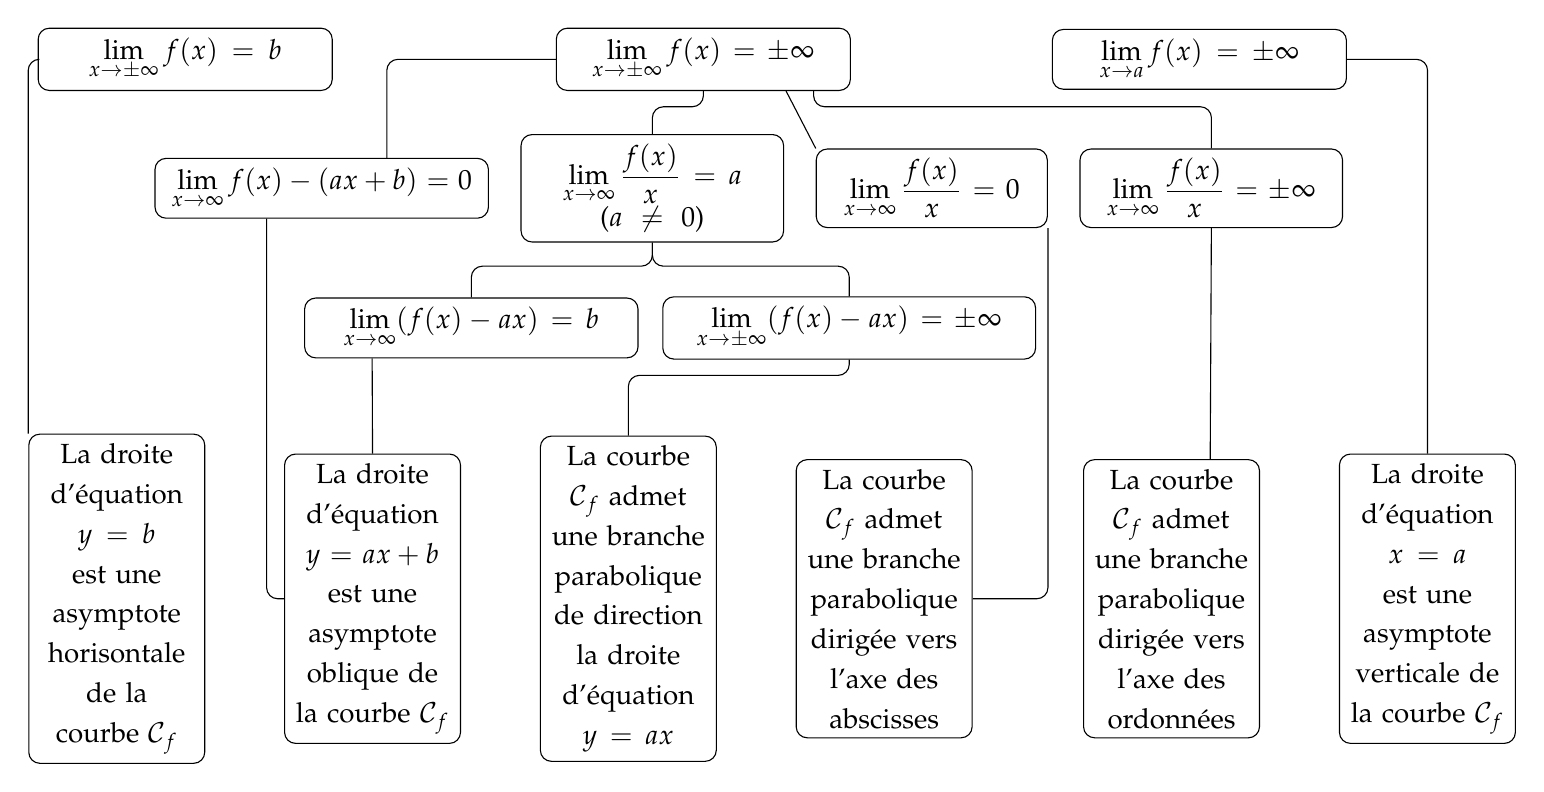
\begin{tikzpicture}[yscale=2,xscale=1.4,rounded corners=4pt]
% xscale et yscale permettent d'ajuster largeur et hauteur
% positionner les nœuds
\node(a) at (-0.7,0)[rectangle,draw,,text width=3.5 cm,,text centered] {$\lim\limits_{x \to \pm\infty} f(x)=b$};
\node(b) at (4,0)[rectangle,draw,,text width=3.5 cm,,text centered] {$\lim\limits_{x \to \pm\infty} f(x)=\pm\infty$};
\node(c) at (8.5,0)[rectangle,draw,,text width=3.5 cm,,text centered] {$\lim\limits_{x \to a} f(x)=\pm\infty$};
%
\node(d) [below left=1.2cm of b ,rectangle,draw,text width=4 cm,text centered] {$\lim\limits_{x \to \infty} f(x)-(ax+b)=0$};

\node(e) [right=0.4cm of d ,rectangle,draw,text width=3.1cm,text centered] {$\lim\limits_{x \to \infty} \dfrac{f(x)}{x}=a$ ($a\neq 0$)};

\node(f) [right=0.4cm of e ,rectangle,draw,text width=2.7cm,text centered] {$\lim\limits_{x \to \infty} \dfrac{f(x)}{x}=0$};

\node(g) [right=0.4cm of f ,rectangle,draw,text width=3.1cm,text centered] {$\lim\limits_{x \to \infty} \dfrac{f(x)}{x}=\pm\infty$};
%
\node(h) [below =1cm of d ,rectangle,draw,text width=4cm,text centered,xshift=1.9cm] {$\lim\limits_{x \to \infty} (f(x)-ax)=b$};
\node(i) [right=0.3cm of h,rectangle,draw,text width=4.5cm,text centered] {$\lim\limits_{x \to \pm\infty} (f(x)-ax)=\pm\infty$};
%
\node(j) [below left=1.35cm of h ,rectangle,draw,text width=2cm,text centered,xshift=-0.3cm] {La droite d'équation $y = b$ est une asymptote horisontale de la courbe $\mathcal{C}_f$};
\node(k) [right=1cm of j ,rectangle,draw,text width=2cm,text centered] {La droite d'équation $y = ax + b$ est une asymptote oblique de la courbe $\mathcal{C}_f$};
\node(l) [right=1cm of k ,rectangle,draw,text width=2cm,text centered] {La courbe $\mathcal{C}_f$ admet une branche parabolique de direction la droite d'équation $y = ax$};
\node(m) [right=1cm of l ,rectangle,draw,text width=2cm,text centered] {La courbe $\mathcal{C}_f$ admet une branche parabolique dirigée vers l'axe des abscisses};
\node(n) [right=1.4cm of m ,rectangle,draw,text width=2cm,text centered] {La courbe $\mathcal{C}_f$ admet une branche parabolique dirigée vers l'axe des ordonnées};
\node(o) [right=1cm of n ,rectangle,draw,text width=2cm,text centered] {La droite d'équation $x = a$ est une asymptote verticale de la courbe $\mathcal{C}_f$};
%%%arrow%%%%%%%%%%%%%%%%%%%
%%%%%%%%%%%%%%%%%%
\draw[midd](a.west)-|(j.north west);
\draw[midd]([xshift=-0.5cm]d.south)|-(k.west);
\draw[midd](b)-|([xshift=2.5cm]d);
\draw[midd](b.south)--([yshift=-0.1cm]b.south)-|(e.north);
\draw[midd ]([xshift=0.75cm]b.south)--(f.north west);
\draw[midd]([xshift=1cm]b.south)--([xshift=1cm,yshift=-0.1cm]b.south)-|(g);
%
\draw[midd](e.south)--([yshift=-0.15cm]e.south)-|(h.north);
\draw[midd](e.south)--([yshift=-0.15cm]e.south)-|(i.north);
\draw[midd](f.south east)|-(m.east);
\draw[midd]([xshift=-0.9cm]h.south)--(k.north);
\draw[midd](i.south)--([yshift=-0.1cm]i.south)-|(l.north);
\draw[midd](g.south)--([xshift=0.35cm]n.north);
\draw[midd](c.east)-|(o.north);
\end{tikzpicture}
}


&\\
\hline
\end{tabular}

\end{document} 